\documentclass[a4paper,12pt]{report}
\usepackage[top=3cm,bottom=3cm,left=3.7cm,right=3cm]{geometry}
\usepackage{setspace}
\doublespacing
\usepackage{subfig}
\usepackage{graphicx}
\usepackage{url}
\usepackage{marvosym}
\usepackage{color}

\begin{document}

\begin{titlepage}
  \begin{center}
    \begin{figure}
      \subfloat{\scalebox{1.0}{\includegraphics{figures/tum-logo.png}}}
      \subfloat{\scalebox{0.23}{\includegraphics{figures/ntu-logo.jpg}}}
    \end{figure}
    \vspace*{1cm}
    \noindent \textbf{\LARGE INVESTIGATION OF TURBULENCE STATISTICS IN SPANWISE OSCILLATING BOUNDARY LAYER} \\
    \vspace*{7cm}
    \noindent \textbf{\large SUNDY WILIAM YAPUTRA} \\
    \vspace*{3cm}
    \noindent \textbf{\large SCHOOL OF MECHANICAL AND AEROSPACE ENGINEERING} \\
    \vspace*{0.5cm} \textbf{2011}
  \end{center}
\end{titlepage}


\begin{titlepage}
  \begin{center}
    \vspace*{2cm}
    \noindent {\LARGE \textbf{Investigation of Turbulence Statistics in Spanwise Oscillating Boundary Layer}} \\
    \vspace*{3cm}
    \noindent {\large \textbf{Sundy Wiliam Yaputra}} \\
    \vspace*{7cm}
    \noindent {\large \textbf{School of Mechanical and Aerospace Engineering}} \\
    \vspace*{0.5cm}
    \noindent A dissertation submitted to Nanyang Technological University \\
    \noindent in partial fulfillment of the requirement for the degree of \\
    \noindent Master of Science (Aerospace Engineering) \\
    \vspace*{0.5cm}
    \noindent \textbf{2011}
  \end{center}
\end{titlepage}


\begin{abstract}
  The role of actively moving boundary layer is very interesting in drag reduction. This project is focused on investigation of turbulent statistics in moving boundary layer. The model used in this project is flat plate with spanwise oscillating movement. To obtain a better insight on the turbulence statistics, Direct Numerical Simulation is used to model the fluid flow.

  In this project, the effect of the surface movement pattern toward drag reduction is observed. The turbulence statistics of interest are velocity profile, turbulence intensities and skin-friction coefficient. To gain a better insight on the moving pattern, comparison is done with related project with different moving pattern.
\end{abstract}

\renewcommand{\abstractname}{Acknowledgements}
\begin{abstract}
  I would like to express my gratitude to the following individuals who have involved in the process of finishing this project, directly and indirectly.
\begin{itemize}
  \item Asst. Prof. Martin Skote for all of his guidances and supervisions to complete this project. I am very grateful because he is willing to work together with me who came to him as a stranger. 
  \item My parents, brother and sister who have supported my decision to join this course. 
  \item Some of classmates in MSc in Aerospace Engineering program.
  \item Last but not least, I would like to express my gratitude to free software and open source communities. This project is completely done by using open source and free softwares. This report was written by using {\bf \LaTeX} in {\bf GNU Emacs}. All the figures were generated by {\bf gnuplot} and the data analysis was done in {\bf GNU Octave}. Ultimately, the whole project was done in {\bf Ubuntu Linux}. Free as in the freedom of speech!!! 
\end{itemize}
\end{abstract}

\pagenumbering{roman}
\tableofcontents
\listoffigures
\listoftables
\pagenumbering{arabic}

\chapter{Introduction}
\section{Background}
Since the depletion of energy resources issue, many efforts have been given to invent new energy resources. Both major inventions are related to the green energy and environment preservation principle. It is believed that these two issues are closely related. 

Energy saving has also been a major research interest in aerospace engineering. Energy saving technologies are not only a breakthrough in environment preservation effort, it also closely related to the economical part of aviation industry. By utilizing these technologies, billions of expenses can be saved from the already expensive cost needed to run an aviation company.

One of the major research interest in aerospace engineering is on the study of drag reduction on aircraft body. Turbulence has been an issue that has been faced by human kind since the invention of first aircraft by Wright brothers at 1903. It is believed that turbulence statistics on aircraft body is considered as the main culprit in increase of drag. 

In general, drag reduction method can be divided into passive and active methods. Major difference between both methods is on its dynamics characteristics. Most of engineering applications adopt passive methods due to its characteristics that do not require external power. However, active methods have gained its own popularity in academical research.

The study of turbulence statistics on aircraft body has been done by many researchers throughout the years. Research mainstreams can be divided into two main categories, computational and experimental. In the past, experimental based researches has been the dominating categories in fluid dynamics. However, with the recent computer technologies development, computational based researches has gained more attention than experimental based researches. 

This project will present a study on turbulent statistics on moving boundary layer in a flat plate. The method used is \emph{Direct Numerical Simulation (DNS)}, which has gained popularity in recent years.

\section{Objective}
The objective of this project is to investigate the effect of wall oscillation on turbulent statistics on near wall region. This project is inspired by the journal published by Viotti and Quadrio~\cite{viotti}, in which the spanwise wall oscillation will be applied with space variation. A case comparison with time variation will also be done, therefore the results obtained from previous final year project~\cite{indra} will be used as comparison.

Since the emphasize of this project is the flow's turbulence statistics, the flow will be plotted only in two-dimensional fields, unlike previous project which include three-dimensional plot. To fulfil the objectives, turbulence statistics investigation done by previous project will be expanded with more statistical parameter.

\section{Scope}
The scope for this projects are:
\begin{enumerate}
\item Investigation of the effect of spanwise wall oscillation with space variation on turbulent statistics
\item Investigation of the comparison of turbulence statistics between spanwise wall oscillation with space variation and time variation
\end{enumerate}

\chapter{Literature Review}
\section{Fundamental Equations of Fluid Dynamics}
The basic principle in the study of fluid dynamics is the prediction of fluid motion around objects. To obtain an accurate prediction on fluid's force and momentum around certain objects, mathematical formulation of the physical behaviour of fluid is required. The fundamental equation of fluid dynamics are~\cite{JB}
\begin{enumerate}
\item Continuity equation (conservation of mass)
\item Momentum equation (conservation of linear momentum)
\item Energy equation (conservation of energy)
\end{enumerate}

The philosophy behind above mathematical formulations is based on the assumption that fluid is a continuous medium. 
 
\subsection{Continuity Equation}
Formulation of fundamental equations of fluid dynamics is done by using finite control volume approach. In finite control volume, a closed volume exists within a finite region of the flow. This volume defines a \emph{control volume}, and a \emph{control surface}. The control volume could be fixed with fluid moving through it or moving with the same fluid particles always inside it. Finite control volume model is illustrated in figure~\ref{fig:control_volume}.
\begin{figure}[h]
  \centering
  \scalebox{0.5}{\includegraphics{figures/control_volume.pdf}}
  \caption{Control Volume (\emph{Source:} Reference~\cite{JA})}
  \label{fig:control_volume}
\end{figure}

The physical principle of mass conservation is mass cannot be created or destroyed. When this principle is applied to fixed control volume, it could be interpreted as
\begin{quote}
Net mass flow out of control volume equals time rate decrease of mass inside control volume~\cite{JA}.
\end{quote}  
Based on this assumption, continuity equation can be formulated to equation~\ref{eq:continuity_1}.
\begin{equation}\label{eq:continuity_1}
  \frac{\partial \rho}{\partial t} + \frac{\partial}{x}\left( \rho u \right) + \frac{\partial}{\partial y}\left( \rho v \right) + \frac{\partial}{\partial z}\left( \rho w \right) = 0
\end{equation}
For steady state condition, equation~\ref{eq:continuity_1} can be simplified to equation~\ref{eq:continuity_2}. 
\begin{equation}\label{eq:continuity_2}
\frac{\partial u}{\partial x} + \frac{\partial v}{\partial y} + \frac{\partial w}{\partial z} = 0
\end{equation}

\subsection{Momentum Equation}
Basic physical principle of momentum equation is Newton's second law, which is force equals time rate of change of momentum. When this physical principle is applied to fixed control volume, the momentum equation can be formulated for x direction (equation~\ref{eq:moment_x}).
\begin{equation}\label{eq:moment_x}
\rho\frac{\partial u}{\partial t} + \rho u\frac{\partial u}{\partial x} + \rho v\frac{\partial u}{\partial y} + \rho w\frac{\partial u}{\partial z} = \rho f_x - \frac{\partial p}{\partial x} + \mu\left(\frac{\partial^2u}{\partial x^2} + \frac{\partial^2u}{\partial y^2} + \frac{\partial^2u}{\partial z^2}\right)
\end{equation}
The same formulation can be done for y and z direction.
\begin{equation}\label{eq:moment_y}
  \rho\frac{\partial v}{\partial t} + \rho u\frac{\partial v}{\partial x} + \rho v\frac{\partial v}{\partial y} + \rho w\frac{\partial v}{\partial z} = \rho f_y - \frac{\partial p}{\partial y} + \mu\left(\frac{\partial^2v}{\partial x^2} + \frac{\partial^2v}{\partial y^2} + \frac{\partial^2v}{\partial z^2}\right)
\end{equation}
\begin{equation}\label{eq:moment_z}
   \rho\frac{\partial w}{\partial t} + \rho u\frac{\partial w}{\partial x} + \rho v\frac{\partial w}{\partial y} + \rho w\frac{\partial w}{\partial z} = \rho f_z - \frac{\partial p}{\partial z} + \mu\left(\frac{\partial^2w}{\partial x^2} + \frac{\partial^2w}{\partial y^2} + \frac{\partial^2w}{\partial z^2}\right)
\end{equation}
Equation~\ref{eq:moment_x}, \ref{eq:moment_y}, and~\ref{eq:moment_z} are known as \emph{Navier -- Stokes} equations. These equations are the fundamental equations to predict force and momentum of fluid around objects.

\section{Boundary Layer Theory}
Although Navier -- Stokes equation is regarded as the fundamental equation in fluid dynamics, until today it has no exact solution. This is because Navier -- Stokes is a nonlinear partial differential equation. Fortunately two main fluids, air and water, have a low viscosity which allow simplification on the fundamental equation. However, this does not justify the omission of viscosity term completely. A complete omission will cause the solution of the simplified equation could not satisfy the complete boundary conditions. 

On 1904, Ludwig L. Prandtl published boundary layer theory. This theory simplify the Navier -- Stokes equations by dividing the flow field into two regions based on its distance from the object's surface, which are~\cite{JB}
\begin{itemize}
\item Viscous boundary layer adjacent to object's surface
\item Inviscid flow outside the boundary layer
\end{itemize}
The schematic of boundary layer can be seen in figure~\ref{fig:boundary_layer}
\begin{figure}[h]
  \centering
  \scalebox{0.5}{\includegraphics{figures/boundary_layer.pdf}}
  \caption{Schematic of boundary layer (\emph{Source:} Reference~\cite{JA})}
  \label{fig:boundary_layer}
\end{figure}

In boundary layer theory, the momentum equation can be simplified into equation~\ref{eq:boundary_layer}.
\begin{equation}\label{eq:boundary_layer}
  \rho u\frac{\partial u}{\partial x}+\rho v\frac{\partial u}{\partial y} = \rho_eu_e\frac{du_e}{dx}+\nu\frac{\partial^2u}{\partial y^2}
\end{equation}

\subsection{Boundary Layer Properties}
Two frequently used boundary layer properties are \emph{displacement thickness} $(\delta^*)$ and \emph{momentum thickness} $(\theta)$~\cite{JA}. Displacement thickness is illustrated in figure~\ref{fig:displ_thick}. Figure on left shows the ideal streamline flow for inviscid case where boundary layer does not exist in object's surface. In this condition, streamline is parallel to object's surface. In constrast to previous condition is actual streamline flow, which is shown by figure on right where boundary layer exists at object's surface. The presence of boundary layer will cause streamline to shift. The distance in which streamline shifted is called displacement thickness. 
   
\begin{figure}[h]
  \centering
  \scalebox{0.5}{\includegraphics{figures/displ_thick.pdf}}
  \caption{Schematic of displacement thickness (\emph{Source:} Reference~\cite{JA})}
  \label{fig:displ_thick}
\end{figure}

Displacement thickness can also be interpreted as index proportional to the ''missing mass flow'' due to the presence of the boundary layer~\cite{JA}. This interpretation is related to mathematical formulation of displacement thickness as can be seen in equation~\ref{eq:displ_thick}
\begin{equation}\label{eq:displ_thick}
\delta^* = \int_{0}^{\delta} \left(1-\frac{u}{u_e}\right)dy
\end{equation}

The second most important boundary layer properties is momentum thickness. Physical interpretation of momentum thickness is momentum loss due to the presence of boundary layer~\cite{PK}. Mathematical formulation of momentum thickness is shown by equation~\ref{eq:momentum}
\begin{equation}\label{eq:momentum}
\theta = \int_{0}^{\delta} \frac{u}{u_e} \left(1-\frac{u}{u_e} \right) dy
\end{equation}

It should be noted that the concept of momentum thickness is useful in prediction of drag coefficient. The relation between momentum thickness and drag coefficient is shown in equation~\ref{eq:cf}, where $L$ is length.
\begin{equation}\label{eq:cf}
C_f = \frac{2\theta}{L}
\end{equation}

\subsection{Boundary Layer in flat plate (Blasius Solution)} 
One of aerodynamics theory application is airfoil. If an infinitesimal length of airfoil's surface is observed, it can be seen as a flat plate. Heinrich Blasius (1908), a student of Prandtl,  performed application of boundary layer theory on a flat plate for the first time on his PhD thesis. This application is known as \emph{Blasius Solution}, which became one of the basic theory behind many boundary-layer theory.

In Blasius equation, a case of incompressible, two-dimensional flow over a flat plate at $0^o$ angle of attack. From such condition, Navier -- Stokes equation is transformed from partial differential equation to \emph{ordinary differential equation} as shown in equation~\ref{eq:blasius}.
\begin{equation}\label{eq:blasius}
2f''' + f f''=0
\end{equation}
Although the Navier -- Stokes equation is simplified to ordinary differential form, the nature of the equation is still nonlinear, which can only be solved numerically.

When above equation is plotted in graph $f'(\eta)=u/u_e$ as a function of $\eta$ (figure~\ref{fig:vel_profile_1}) it can be seen that $u$ will change when the flow move downstream. However, when plotted in graph versus $\eta$ (figure~\ref{fig:vel_profile_2}), it can be seen that $u = u(\eta)$ profile is the same as the flow progress downstream. This \emph{similarity} is called \emph{self-similarity solution}~\cite{JA}. Self-similar profile can only be found on a certain type of flows. Boundary layer profile for flows over an arbitrary body are \emph{nonsimilar}.
\begin{figure}[h]
  \centering	
  \scalebox{0.5}{\includegraphics{figures/vel_profile_1.pdf}}
  \caption{Incompressible velocity profile for a flat plate; solution of the Blasius equation.(\emph{Source:} Reference~\cite{JA})}
  \label{fig:vel_profile_1}
\end{figure}

\begin{figure}[h]
  \centering
  \scalebox{0.5}{\includegraphics{figures/vel_profile_2.pdf}}
  \caption{Velocity profile in physical and transformed space, demonstrating the meaning of self-similar solution.(\emph{Source:} Reference~\cite{JA})}
  \label{fig:vel_profile_2}
\end{figure}

\subsection{Laminar boundary layer}
Boundary layer could be divided into two areas, \emph{laminar}and \emph{turbulent} boundary layer. In laminar boundary layer area, the momentum transfer in the direction perpendicular to the flow happens in molecular/microscopic scale. Because of molecular movement, \emph{slower-moving} fluid particles from lower layer will move upward and slowing the particles in upper layer. In other side, when upper layer \emph{faster-moving} fluid particles moves downward, it will accelerate the lower layer fluid particles~\cite{JB}. Figure~\ref{fig:comparison} illustrates the phenomena explained before.

\begin{figure}
  \centering
  \scalebox{0.7}{\includegraphics{figures/comparison.pdf}}
  \caption{(a) Laminar, (b) Turbulent}
  \label{fig:comparison}
\end{figure}

The laminar boundary layer properties for Blasius equations can be obtained through numerical calculation of equation~\ref{eq:blasius}. Some of the important properties are skin friction coefficient (equation~\ref{eq:laminar_cf}) and boundary layer thickness (equation~\ref{eq:laminar_blthickness}).

\begin{equation} \label{eq:laminar_cf}
  C_f = \frac{1.328}{\sqrt{Re_c}}
\end{equation}

\begin{equation} \label{eq:laminar_blthickness}
  \delta = \frac{5.0x}{\sqrt{Re_x}}
\end{equation}

\subsection{Turbulent boundary layer}
Transformation of laminar boundary layer to turbulent boundary layer does not takes place instantly. \emph{Transition} area exists between both boundary layers. The length of transition area can be the same as laminar boundary layer length. The physical principle behind the laminar boundary layer transformation to turbulent can be described as follow. The boundary layer formed in object's surface is subjected to numerous disturbance, e.g. surface roughness, temperature irregularities, background noise, etc. For some flow, these disturbances are damped which make boundary layer stay laminar. However, for some other type of flow, the disturbances are amplified and the boundary layer becomes turbulent. 

In constrast with laminar boundary layer, in turbulent boundary layer the momentum transfer takes place in a macroscopic scale. Thus, in addition to laminar shear stress, a large \emph{turbulent shear stress} exist along the same direction.

Due to slower-moving fluid particles near the wall are transported well upward, turbulent boundary layer has a relatively large thickness. Turbulent boundary layer also has larger shear stress than a laminar boundary layer. This is because faster-moving fluid particles are transported toward the wall and produce relatively high velocity for the fluid particles near the surface.

Since turbulent flow is highly unpredictable, turbulent boundary layer properties for flat plate are obtained from empirical data. Some important properties are shown in equation~\ref{eq:turbulent_cf} and~\ref{eq:turbulent_blthickness}

\begin{equation} \label{eq:turbulent_cf}
  C_f = \frac{0.074}{\sqrt{Re_c^{1/5}}}
\end{equation}

\begin{equation} \label{eq:turbulent_blthickness}
  \delta = \frac{0.37x}{\sqrt{Re_x^{1.5}}}
\end{equation}

When the boundary-layer thickness for turbulent boundary layer (equation~\ref{eq:turbulent_blthickness}) is compared with laminar boundary layer (equation~\ref{eq:laminar_blthickness}), it could be seen that turbulent boundary-layer thickness grow more rapidly than its laminar counterpart. In other side, turbulent boundary layer also produces larger wall friction coefficient, as can be seen from the comparison between equation~\ref{eq:turbulent_cf} and~\ref{eq:laminar_cf}.

\section{Computational Fluid Dynamics}
Although boundary layer theory greatly simplify Navier -- Stokes equation, there are still no exact analytical solution for the fundamental equations. The main hurdle is because Navier -- Stokes equation is a nonlinear partial differential equation, which has no exact solution exist until today. 

Computational Fluid Dynamics (CFD) is a study of fluid mechanics that heavily utilize numerical analysis and algorithms to solve and analyze fluid dynamics problems~\cite{Wiki}. In contrast with solution provided by analytical solution, CFD result is a collection of numbers that represents the approximate solution of Navier -- Stokes equation. 

With advancement of computer technology, CFD has gained its popularity in engineering application. Many engineering problems that cannot be done by experiment method, has been solved with CFD methods. Some of the advantages of CFD method are 
\begin{itemize}
\item Less time and financial resources needed in solving problem.
\item CFD methods have solve many problems that previously cannot be done by
experimental methods due to environment constraints etc. 
\end{itemize} 

The basic principle of numerical analysis is to breakdown continuous mathematical function into algebraic equation. This can be done through discretization method, which is one of the important aspect in Computational Fluid Dynamics. There are few discretization methods used in CFD, e.g. \emph{Finite Difference Method}, \emph{Finite Element Method (FEM)}, \emph{Finite Volume Method}, spectral method, etc.

\subsection{Direct Numerical Simulation}  
In fluid dynamics, study of turbulence is considered as one of the interesting subject. Turbulence is largely consist of mixture between order and chaos and possess a wide range of length and time scales~\cite{parviz}. Due to the limitation of past computer technology, it was impossible to solve turbulence problem by using only Navier -- Stokes equation. Hence, turbulence modelling was introduced as a complement, e.g.  RANS (Reynolds-Averaged Navier -- Stokes) and LES (Large Eddy Simulation). Turbulence model can be used to approximate or to average the number of turbulent statistics in the flow. By using turbulence model, turbulent flow computation can be simplified.  However, with the increase of flow complexity, a better computation tool is needed.

\emph{Direct Numerical Simulation (DNS)} is computational fluid dynamics simulation method where Navier -- Stokes equation is solved without turbulence model. Since the computation is done without any simplification, DNS's accuracies are very high. To ensure that the computation able to contain all the significant turbulent statistics, DNS method requires a very large scale of computation.

With regards to its computation scale, DNS method is very time consuming. Even with the state of art computer technology, it is still limited to flow with relatively low Reynolds numbers and geometrically simple domain. Although it provides a very detailed information,  DNS result is deemed superfluous and too expensive for commercial purpose. On the other hand, DNS has gained a lot of attention in academical research and has been applied as research tool to some applications. Some example on which DNS has been applied are~\cite{ferziger}:

\begin{itemize}
\item Understanding the mechanism of turbulence production, energy transfer, and dissipation in turbulent flows
\item Simulation of the production of aerodynamics noise
\item Understanding the effects of compressibility on turbulence
\item Understanding the interaction between combustion and turbulence
\item Controlling and reducing drag on a solid surface
\end{itemize}

For simple geometry, DNS has been done by using spectral method to discretize Navier -- Stokes equation~\cite{chung}. The streamwise and spanwise directions are discretized by using \emph{Fourier series} and wall-normal direction by \emph{Chebysev polynomials} or \emph{B-splines}. However, spectral method applications are only limited to simple geometry. For complex geometries, DNS has been carried out by using finite difference method with less accuracy. In recent years, the application of finite element method and unstructured grid are being explored~\cite{parviz}.

\subsection{Spectral method}
Spectral method are a class of spatial discretizations for differential equations~\cite{canuto}. Spectral method consist of basis functions which will provide approximate solutions. The choice of basis functions in spectral method is the feature that distinguish it from other discretization methods such as finite element method.  Finite element method's basis function acts as \emph{local} functions, which are polynomials with low degree. In contrast with finite element method, spectral method's basis functions acts as \emph{global} functions, which are polynomials with high degree, e.g. Fourier series, Chebysev polynomials, etc~\cite{boyd}. The choice of basis functions provide pro and cons for both methods. Finite element method can be fitted to complex geometries enough flexibility, however it suffers for low accuracy. On the other hand spectral method produce a high accuracy, but its applications are limited only to regular and smooth geometry.

Although spectral method's error converges faster than other discretization methods, e.g. finite difference method, it is not the best method available. The drawbacks of spectral method are:
\begin{itemize}
\item Spectral method's algorithms are more difficult to program
\item More expensive with the increase of degree of freedom 
\item Low performance in complex geometries
\end{itemize}
 
\subsection{Verification and Validation}
Software used in this project is \emph{Simson}. This software is developed in Royal Institute of Technology, Sweden. This software has been used in several research projects, e.g. Skote et al.~\cite{skote-1}, Henkes et al.~\cite{skote-2} and etc. In Skote et al.~\cite{skote-1}, the numerical result on turbulent statistics of zero pressure gradient and adverse pressure gradient show an agreement with the experimental result. In Henkes et al.~\cite{skote-2} a few turbulent models are evaluated. From the few methods, Differential Reynolds Stress Model (DRSM) shows good agreement with experimental results, while algebraic model and $k-\omega$ models show reasonably accurate result. However $k-\epsilon$ model gives a rather large deviations for strong adverse pressure gradients. 
\chapter{Methodology}
\section{Hardware and Protocol}
The computational data for this project is obtained by using high performance cluster in High Performance Computing Center in NTU (HPC-NTU). The connection to HPC-NTU is done through SSH (Secure Shell) protocol.

\section{Software}
Tools used for this project are \emph{Simson and gnuplot}. Simson is used in pre-processing and post-processing stages, while gnuplot is used only in pre-processing stage. Complete project workflow is illustrated in figure~\ref{fig:method}.
\begin{figure}[h]
  \setlength{\unitlength}{0.6mm}
  \centering 
  \begin{picture}(80,250)\thicklines
    \put(40,220){\framebox(40,20){fsc}}
    \put(60,220){\vector(0,-20){20}}
    \put(40,180){\framebox(40,20){bls}}
    \put(60,180){\vector(0,-25){25}}
    \put(40,135){\framebox(40,20){bla}}
    \put(60,135){\line(0,-15){15}}
    \put(30,120){\line(60,0){60}}
    \put(30,120){\vector(0,-20){20}}
    \put(90,120){\vector(0,-20){20}}
    \put(10,80){\framebox(40,20){rit}}
    \put(70,80){\framebox(40,20){pxyst}}
    \put(90,80){\vector(0,-20){20}}
    \put(70,40){\framebox(40,20){gnuplot}}
    \put(-45,170){\dashbox{1}(175,80)[lt]{\bf \scriptsize Post--processing}}
    \put(-45,130){\dashbox{1}(175,30)[lt]{\bf \scriptsize Processing}}
    \put(-45,30){\dashbox{1}(175,80)[lt]{\bf \scriptsize Pre--processing}}
    \thinlines\put(0,75){\framebox(120,185)[rt]{\bf \scriptsize Simson}}
  \end{picture}
  \caption{Project workflow}
  \label{fig:method}
\end{figure}

Simson is a CFD solver package developed by Royal Institute of Technology, Sweden. It implements spectral integration technique to solve Navier -- Stokes equation for incompressible channel and boundary flows~\cite{Simson}. Simson's code is written in Fortran 77/90, and is supported by OpenMP and MPI interface to support parallel programming. The code can be used as direct numerical simulation (DNS) and large eddy simulation (LES) solver. Simson's parts used in this project are {\bf bla} (main program), {\bf rit} (program to plot solution from complete velocity fields), and {\bf pxyst} (program to plot \emph{xy-statistics}). Complete informations of softwares used are listed in table~\ref{tab:software}.
\begin{table}[h]
  \centering
  \begin{tabular}[h]{c l l}
    \hline\hline
    No. & Software & Information \\
    \hline
    1 & fsc & Calculate velocity profile \\
    2 & bls & Calculate initial velocity field \\
    3 & bla & Main processing software \\ 
    4 & rit & Plot velocity field \\ 
    5 & pxyst & Plot statistics data  \\ 
    6 & gnuplot & Used to produce graphics\\
    \hline
  \end{tabular}
  \caption{List of softwares used in the project}
  \label{tab:software}
\end{table}

 \subsection{Processing}
The processing stage is done by using main program {\bf bla}.
 
\subsection{Pre--processing}
 Main program {\bf bla} requires velocity field as input files. This file is generated by program {\bf bls}. Velocity field generated by {\bf bls} consists of a basic laminar flow and a range of different disturbances, e.g. localized disturbance, waves and random noise. In some type of flow, laminar base flow profile is not given analytically. Therefore a velocity profile file must be generated by using program {\bf fsc}.

 {\bf bla} can be run in serial mode and parallel mode. In serial mode, {\bf bla} only requires a single processor to run the simulation. To run in parallel mode {\bf bla} is supported with MPI and OpenMP interface. Since {\bf bla} is used in batch mode, it has no interactive input. It can be configured during compilation by using file {\bf par.f} and runtime by using {\bf bla.i} file.

{\bf bla} consists of \emph{subroutines} that form the main program. In this project, subroutines that will be given special attention are {\bf rparambl}, {\bf linearbl} and {\bf cwallbc}. For a complete listing of {\bf bla's} subroutine, pelase refer to Simson's User Guide~\cite{Simson}.

\subsection{Post--processing}
{\bf rit} and {\bf pxyst} are Simson's programs used in post-processing stage. {\bf rit} is used to generate various graph of velocity field in Simson. It requires velocity field  ({\bf .u}) input files.

{\bf pxyst} can be used to plot of both time and spanwise averaged data. It generates plot for both raw statistical data and derived quantities. {\bf pxyst} is also used to generate various special plots of the mean flow, such as boundary layer thickness and skin friction. To run {\bf pxyst},  statistics ({\bf .stat}) files are required  as input.

The comparison between statistics data could not be done by using {\bf pxyst}. In order to gain more insight of flow behaviour, results obtained through {\bf pxyst} are saved in the form of data file and plotted by using gnuplot.

\chapter{Implementation of Wall Oscillation}
\section{Mathematical Formulation of Wall Oscillation}
The wall oscillation model is applied along the streawise x-direction as shown by figure~\ref{fig:wall_oscill}.
\begin{figure}[h]
  \centering
  \scalebox{0.5}{\includegraphics{figures/wall_oscill.pdf}}
  \caption{Wall oscillation model}
  \label{fig:wall_oscill}
\end{figure}
Since the wall oscillation only occurs on particular region, a profile function $f(x)$ is inserted to the wall oscillation model to act as a filter. The complete mathematical formulation of the wall oscillation can be seen in equation~\ref{eq:wall_oscill}.
\begin{equation}\label{eq:wall_oscill}
  w|_{y=0} = amp\cdot f(x)\cdot\sin (x_{omeg}x)
\end{equation}
With profile function $f(x)$ is formulated in equation~\ref{eq:prof_func}
\begin{equation}\label{eq:prof_func}
  f(x)=S\left(\frac{x-x_{start}}{x_{rise}}\right)-S\left(\frac{x-x_{end}}{x_{fall}}+1\right)
\end{equation}

The terms $amp,x_{start},x_{rise},x_{end},x_{fall}$ and $x_{omeg}$ are represented by the runtime parameter \emph{amp,xstart,xrise,xfall} and \emph{xomeg} respectively. Each terms description is given in table~\ref{tab:runtime}.
\begin{table}[h]
  \centering
  \begin{tabular}{|l|c|l|c|}\hline
    Runtime Parameter & Variable & Description & Data Type \\ \hline
    amp & wp1 & Maximum Amplitude & real \\
    xstart  & wpds1 & Start position of wall oscillation & real \\
    xend & wpds2 & End position of wall oscillation & real \\
    xrise & wpds3 & Rise length of wall oscillation & real \\
    xomeg & wpdds1 & Position variation & real \\ \hline
  \end{tabular}
  \caption{Correspondence between Runtime Parameter in bla.i and Variables in Subroutine rparambl}
  \label{tab:runtime}
\end{table}

$S(x)$ is a ''continuous'' step function which can be formulated in equation~\ref{eq:step_func}.
\begin{equation} \label{eq:step_func}
  S(x) = \left\{ 
    \begin{array}{lr}
      0, & x \leq 0 \\
      1/\left(1/1+e^{(1/(x-1)+1/x)}\right), & 0 < x < 1 \\
      1, & x \geq 1
    \end{array}
  \right.
\end{equation}
Schematic of function $S(x)$ is shown in figure~\ref{fig:step_func}.
\begin{figure}[h]
  \centering
  \scalebox{0.7}{\includegraphics{figures/fx.pdf}}
  \caption{Schematic picture of function $S(x)$}
  \label{fig:step_func}
\end{figure}

\section{Computational Method}
The implementation of wall boundary condition to Simson is done by modification of the main program {\bf bla} and several subroutines, which are:
\begin{itemize}
\item {\bf cwallbc}, subroutine to set wall boundary condition,
\item {\bf rparambl}, subroutine used to link main program {\bf bla} and {\bf bla.i} that contains runtime parameters, and \item {\bf linearbl}, subroutine used to apply boundary condition
\end{itemize}

\subsection{Modification of subroutine rparambl}
Subroutine rparambl is used to read the runtime parameters stored in bla.i and relay the informations to bla as inputs needed during simulation. When new boundary conditions or variables are declared in cwallbc, the same boundary conditions and new variable need to be declared in rparambl as well.

Implementation of the new boundary layer model is done by setting a new value to wbci ($wbci = 4$). By setting a new value to wbci, a new boundary layer model is created in Simson. Other change done in rparambl is the initialization of new variables. These variables are runtime parameters needed by bla as inputs to simulate the new boundary layer condition. The list of new parameters declared in rparambl is available in table~\ref{tab:runtime}. Detail changes of subroutine rparambl is explained in appendix~\ref{app:bla_change}. The value of both wbci and new variables are assigned in bla.i as runtime parameters.
 
\subsection{Modification of subroutine cwallbc}
Subroutine cwallbc is used to set the boundary condition in Simson. Since the wall oscillation model is residing in cwallbc, the subroutine has been changed substantially. To implement the wall oscillation model, new variables are declared in cwallbc, which are: \emph{dnx, fstcm denc, r, xst, xen, imin, xendc, i, etc}. Some variables declared in last project ($wbci = 3$) are also included in the formulation, which are: \emph{walloscur, walloscui, walloscwr,and walloscwi}. Variables exist in original code, \emph{alfa} and \emph{beta}, are also included.

The next changes in cwallbc subroutine is the generation of the $w|_{y=0}$, which is represented by the variables \emph{wlwr} and \emph{wlwi}. Previous project ($wbci = 3$) manage to utilize the existing code from $wbci = 1$ successfully. However the same result could not be produce when used in the new wall oscillation model. When the existing code is applied to the new wall oscillation model, the resulting graphic show the there are discontinuities in the middle of the computational box. The discontinuity is caused by the generation of fringe function in the odd and even space respectively. Therefore, a difference approach is used to apply the wall oscillation model to the boundary condition. The major changes done in the new approach is the conversion of \emph{xstart} and \emph{xend} to channel code. 

Although previous project's approach could not be used for generation of $w|_{y=0}$, the transformation of variables \emph{wlwr} and \emph{wlwi} from real to half complex in x-directions is done by using the code from previous project. The same code is also used to do the normalization of variables \emph{wlwr} and \emph{wlwi}. The detail of all of the change in subroutine cwallbc is given in appendix~\ref{app:bla_change}.

\subsection{Modification of subroutine linearbl}
The boundary conditions are located in subroutine linearbl. The changes done In linearbl, different boundary condition are set on even/odd points and setting new boundary conditions for wavenumber zero. The detail of change is listed in appendix~\ref{app:bla_change}.

\subsection{Modification of main program bla} 
Main program bla is the main program where the operation of all subroutines are combined. The implementation of wall oscillation model to Simson requires some changes in main program bla as well. These changes are the declaration of new variables used in subroutine cwallbc and linearbl, which are wlwr, wlwi, walloscur, walloscui, wallloswr and walloscwi for all oscillation as a global variable. 

\section{Testing of Wall Oscillation}
To ensure the validity of the code, a test is performed to check the wall oscillation profile. Since no data will be collected during the test, the simulations are done in small scale. The size of the computational box is given by: $xl=112$, $yl=34$ and $zl=16$ which are set in \emph{bls.i}. The spectral number for \emph{x, y} and \emph{z}-direction is given by $nx =120, ny=61 \mbox{ and } nz=48$ which are set in \emph{par.f}. These parameters are the resolutions of the simulation.

The test simulations are performed in four cases according to the location of the wall oscillations. The first case is done with $xstart = 0$ and $xend = 40$, the second case is done with $xstart=40$ and $xend=80$, third case is done with $xstart=80$ and $xend = 112$ and the last case is done with $xstart = 0$ and $xend = 112$. All simulations are done with $xomeg = 0.38$, $xrise=20$, $xfall=20$ and $amp=0.5$.

The results of the test simulations can be seen in figure~\ref{fig:w(f(x))-test}. Since the test is done to test the wall oscillation profile, the simulation results are plotted as $w$ component as function of $x$ with $y=0$ ($w(f(x))|_{y=0}$).

\begin{figure}[!h]
  \centering
  \subfloat[]{\label{fig:w(f(x))-1}\scalebox{0.7}{\includegraphics{figures/w(f(x))-1.pdf}}} \\
  \subfloat[]{\label{fig:w(f(x))-2}\scalebox{0.7}{\includegraphics{figures/w(f(x))-2.pdf}}}
  \caption{Two dimensional contour plot of wall oscillation tested in various region at $y=0$: (a) $w(f(x))|_{y=0} \mbox{ at } xstart = 0 \mbox{ and } xend = 40$, (b) $w(f(x))|_{y=0} \mbox{ at } xstart = 40 \mbox{ and } xend = 80$, (c) $w(f(x))|_{y=0} \mbox{ at } xstart = 80 \mbox{ and } xend = 112$}
  \label{fig:w(f(x))-test}
\end{figure}

\begin{figure}[!h]
\ContinuedFloat
\centering
   \subfloat[]{\label{fig:w(f(x))-3}\scalebox{0.7}{\includegraphics{figures/w(f(x))-3.pdf}}}\\
   \subfloat[]{\label{fig:w(f(x))-4}\scalebox{0.7}{\includegraphics{figures/w(f(x))-4.pdf}}}
   \caption{Two dimensional contour plot of wall oscillation tested in various region at $y=0$: (a) $w(f(x))|_{y=0} \mbox{ at } xstart = 0 \mbox{ and } xend = 40$, (b) $w(f(x))|_{y=0} \mbox{ at } xstart = 40 \mbox{ and } xend = 80$, (c) $w(f(x))|_{y=0} \mbox{ at } xstart = 80 \mbox{ and } xend = 112$, (d)  $w(f(x))|_{y=0} \mbox{ at } xstart = 0 \mbox{ and } xend = 112$}
 \end{figure}

\section{Simulation Parameters}
For comparison purpose, the simulation's parameters used are similar to the parameters used in previous final year project~\cite{indra}. The parameters are listed in the table~\ref{tab:params}.
\begin{table}[h]
  \centering
  \begin{tabular}[h]{l c}
    \hline\hline
    Parameters & Value\\
    \hline
    $x_{start}$ & 250.0 \\
    $x_{end}$ & 482.7 \\
    $Re$ & 400 \\
    \hline
  \end{tabular}
  \caption{Simulation parameters}
  \label{tab:params}
\end{table}
\chapter{Results and Discussion}
\section{Flow Visualization}
The simulation is done with $xstart = 250$, $xend = 482.7$ and the spatial oscillation occurs at wavelength of $\lambda = 58$. The graphical representation are shown by figure~\ref{fig:w(f(x))} and~\ref{fig:w(x,z)}. 
\begin{figure}[h]
  \centering
  \scalebox{0.7}{\includegraphics{figures/w(f(x))_t7000.pdf}}
  \caption{Two dimensional contour plots of wall oscillation at $y=0:w(f(x))|_{y=0}$ with \emph{xstart} = 250, \emph{xend} = 482.7 and $\lambda$ = 58}
  \label{fig:w(f(x))}
\end{figure}

\begin{figure}[h]
  \centering
  %\scalebox{0.7}{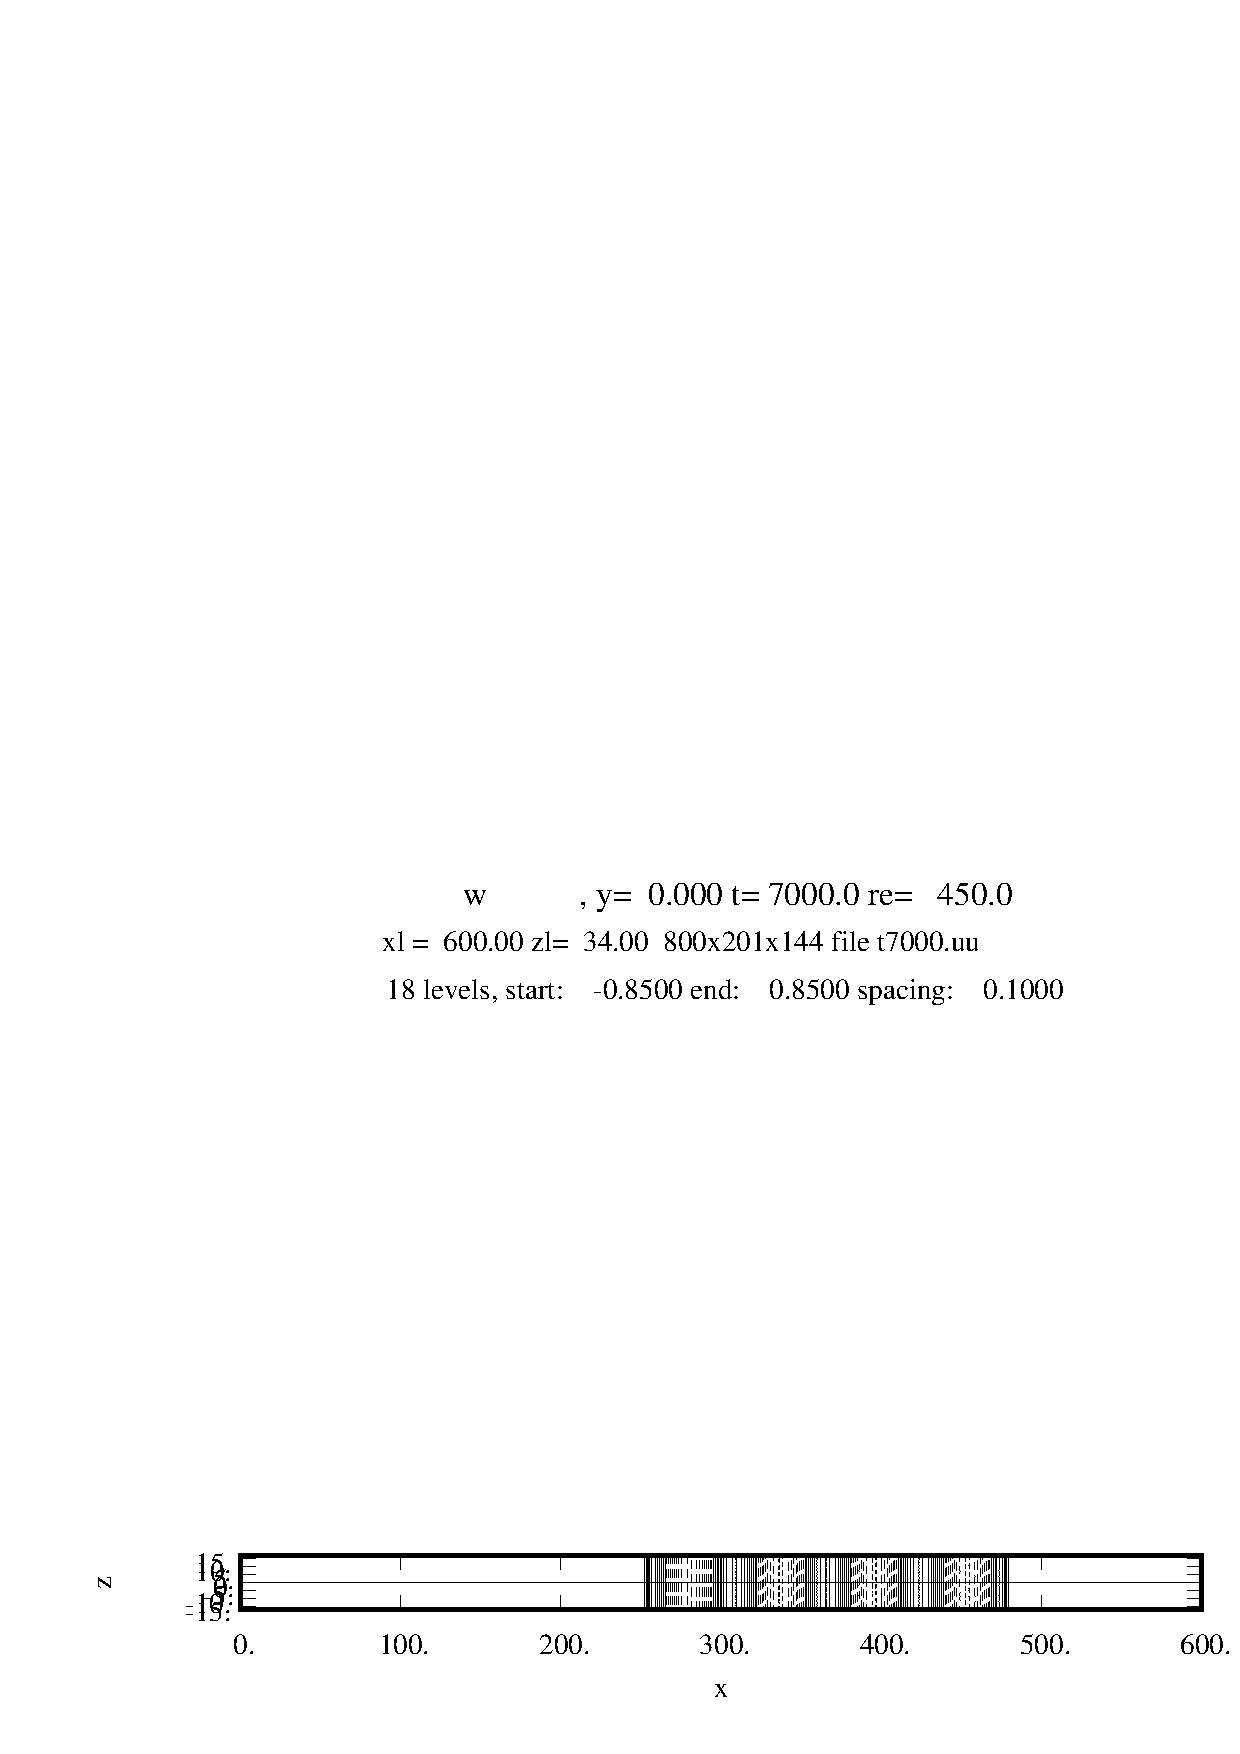
\includegraphics{figures/w(x,z).pdf}}
  \includegraphics[width=15cm]{figures/w_4.pdf}
  \caption{Two dimensional contour plots of wall oscillation at $y=0:w(x,z)|_{y=0}$ with \emph{xstart} = 250, \emph{xend} = 482.7 and $\lambda$ = 58}
  \label{fig:w(x,z)}
\end{figure}

\subsection{Streamwise Velocity Field}
Streamwise velocity field refers to the \emph{x}-component of the velocity vector of the fluid. It has the direction parallel to the plate along the fluid stream. In standard notation, it is represented by variable \emph{u}. In this project, only two-dimensional contour plots will be given.

Since there are great ratio difference between x and y-direction, an equal ratio plot will not produce good flow visual. To improve the visibility, y-direction is stretched to accommodate the length of x-direction.

In this simulation, the wall oscillation is started from $xstart = 250$ to $xend = 487.2$. In accordance with the step function, the inflow and outflow of the computational box is laminar flow. This is followed by the transition area, which is shown by the slope on the function. The flow image is plotted by using 20 contour. Two dimensional contour plot of streamwise velocity field in plane $z=0$ at $t = 19600$ can be seen in figure~\ref{fig:u(x,y)}.

\begin{figure}[!h]
  \centering
  \scalebox{0.7}{\includegraphics{figures/u(x,y)_t19600.pdf}}
  \caption{Streamwise velocity field at $t = 19600$ }
  \label{fig:u(x,y)}
\end{figure}

In the area where the wall oscillation is applied, it can be seen that the velocity field are looser than its counterpart. However, in the near wall region, the velocity field has no significant change.

\subsection{Wall Normal Velocity Field}
Wall normal velocity field refers to the \emph{y}-component of the velocity vector of the fluid. It has direction perpendicular to the plate. In standard notation, it is represented by variable \emph{v}.

Since there are great ratio difference between x and y-direction, an equal ratio plot will not produce good flow visual. To improve the visibility, y-direction is stretched to accommodate the length of x-direction.

In this simulation, the wall oscillation is started from $xstart = 250$ to $xend = 487.2$. The flow image is plotted by using 20 contour. Two dimensional contour plot of wall normal velocity field in plane $z=0$ at $t = 19600$ can be seen in figure~\ref{fig:v(x,y)}.

\begin{figure}[!h]
  \centering
  \scalebox{0.7}{\includegraphics{figures/v(x,y)_t19600.pdf}}
  \caption{Wall normal velocity field at $t = 19600$}
  \label{fig:v(x,y)}
\end{figure}

The introduction of wall oscillation in wall normal direction will thin away at the near wall region. This is shown by the difference of space between left and right part of computational box, in which more space can be found at $x=250-500$ region.

\subsection{Spanwise Velocity Field}
Wall normal velocity field refers to the \emph{z}-component of the velocity vector of the fluid. It has directions parallel to the plate and parallel to the width dimension of the plate. In standard notation, it is represented by variable \emph{w}.

Since there are great ratio difference between x and y-direction, an equal ratio plot will not produce good flow visual. To improve the visibility, y-direction is stretched to accommodate the length of x-direction.

In this simulation, the wall oscillation is started from $xstart = 250$ to $xend = 487.2$. The flow image is plotted by using 20 contour. Two dimensional contour plot of spanwise velocity field in plane $z=0$ at $t = 19600$ can  be seen in figure~\ref{fig:w(x,y)}.

\begin{figure}[!h]
  \centering
  \scalebox{0.7}{\includegraphics{figures/w(x,y)_t19600.pdf}}
  \caption{Spanwise velocity field at $t = 19600$}
  \label{fig:w(x,y)}
\end{figure}

In spanwise velocity field it can be seen the application of wall oscillation will cause the velocity field to thicken in the near wall region. This is shown by the flow lines which stack together at $x=250-500$ compared to the flow lines at $x=0-250$ where more space can be found in the near wall region.

\subsection{Streamwise Velocity Fluctuations}
The fluctuation of streamwise velocity field is obtained by applying gaussian anisotropic high-pass filter to the streamwise velocity field. This filter removes the mean value of the streamwise velocity, hence displaying the low-speed and high-speed streak of the streamwise velocity.

Figure~\ref{fig:svl_0-250} shows the streamwise velocity fluctuations at $x = 0 - 250$. It can be seen that when the flow is not exposed to oscillation, the box is full of fluctuation. This is in contrast with the condition shown in figure~\ref{fig:svl_250-500}. At position $x = 250 -500$, when the flow is exposed to oscillation, the box is has less fluctuation compared to the previous position. With decreasing number of fluctuations it can be assumed that the drag at that location is reduced. This assumption will be further discussed in the next section.  

\begin{figure}[!h]
  \centering
  \subfloat[$x=0 - 250$]{\label{fig:svl_0-250}\scalebox{0.7}{\includegraphics{figures/w(x,z)_0-250.pdf}}} \\
  \subfloat[$x=250 - 500$]{\label{fig:osc_0-250}\scalebox{1.05}{\includegraphics{figures/w_x_0-250.pdf}}}
  \caption{Two dimensional contour plots of streamwise velocity field fluctuations at plane $y=1$ at $t= 19600$: -- $u=-0.05$; - - $u=0.05$}
  \label{fig:stream_vel_fluct_0-250}
\end{figure}

\begin{figure}[!h]
  \centering
  \subfloat[$x=0 - 250$]{\label{fig:svl_250-500}\scalebox{0.7}{\includegraphics{figures/w(x,z)_250-500.pdf}}} \\
  \subfloat[$x=250 - 500$]{\label{fig:0sc_250-500}\scalebox{1.05}{\includegraphics{figures/w_x_250-500.pdf}}}
  \caption{Two dimensional contour plots of streamwise velocity field fluctuations at plane $y=1$ at $t= 19600$: -- $u=-0.05$; - - $u=0.05$}
  \label{fig:stream_vel_fluct_250-500}
\end{figure}

\section{Drag reduction}
The investigation of the effect of wall oscillation on drag reduction can be done through skin friction coefficient. The mathematical formulation for skin friction coefficient is shown by equation~\ref{eq:skin_friction}. 
\begin{equation}\label{eq:skin_friction}
  C_f = 2\left(\frac{u_\tau}{U_\infty}\right)
\end{equation}
The friction velocity ($u_\tau$) can be calculated from the mean streamwise velocity gradient at the wall, which is shown in equation~\ref{eq:u_tau}
\begin{equation}\label{eq:u_tau}
  u_\tau = \sqrt{v\left.\frac{\partial u}{\partial y}\right|_{y=0}}
\end{equation} 

Figure~\ref{fig:cf_all} shows the skin friction coefficient $(C_f)$ as function of streawise coordinate $(x)$. To avoid the confusion caused by the numerical effects, the graph is shown in the range of $x=150$ to $x=500$. In figure~\ref{fig:cf_all}, the skin friction coefficient of undisturbed (---) is compared with the simulation results after 200, 400, 600, 800 ($\cdots$) and the total cycles (\textbf{---}).  

\begin{figure}[!h]
  \centering
  \scalebox{1.1}{\includegraphics{figures/cf-total-all.pdf}}
  \caption{Skin friction coefficient (undisturbed (---), 200, 400, 600 and 800 cycles ($\cdots$), total cycles (\textbf{---})). It can be seen that the application of wall oscillation will reduce the skin friction coefficient significantly. The skin friction coefficient is reduced gradually with the increase of time.}
  \label{fig:cf_all}
\end{figure}

Figure~\ref{fig:cf_all} shows that the skin coefficient friction shows reduction at $x=250$ where the oscillation start. At the end of wall oscillation $(x=482.7)$, the skin friction coefficient will gradually return to its original position. The number of cycles also give significant effects to the drag reduction. It can be seen that the drag reduction given by 200 cycles is less than the 600, etc. With the increasing number of cycles, the reduction will eventually reach its constant value which is shown by the results from total cycles (---). 

To see the difference between the effect of spanwise wall oscillation with space variation and time variation, simulation results from previous final year project (---) is compared with current simulation results ($\cdots$). Figure~\ref{fig:cf_compare} shows the comparison of skin friction coefficient between the undisturbed case, time variation and space variation simulations results. Similar to figure~\ref{fig:cf_all}, the simulation box is limited in the range of $x=150$ to $x=500$ to avoid the effect caused by the numerical scheme.

\begin{figure}[!h]
  \centering
  \scalebox{1.1}{\includegraphics{figures/cf-total-compare.pdf}}
  \caption{Skin friction coefficient comparison(temporal (\Cutline), spatial (---)). The spatial variation produce more skin friction coefficient reduction than temporal variation. Note that a pattern similar to wall oscillation exist in spatial variation curve.}
  \label{fig:cf_compare}
\end{figure}

From figure~\ref{fig:cf_compare}, it can be seen that the spanwise wall oscillation with space variation result more drag redu ction compared to time variation (previous case). An interesting behaviour is also shown by the spatial variation simulation results. In the region where the wall oscillation is applied, there is certain pattern that resembles the wall oscillation. This pattern is not found in the simulation results from previous final year project (wall oscillation with time variation). The cause of this pattern is assumed as the effect of the wall oscillation with spatial variation. This assumption is supported by the occurrence with same pattern in other simulation results (200, 400, 600 and 800 cycles) shown in figure~\ref{fig:cf_all}. 

It can be seen that the pattern will gradually form a fixed pattern with the increasing cycles, which is shown by figure~\ref{fig:cf_zoom}. The simulation result with 200 cycles shows a strong pattern, which gradually decrease with the increase of cycles.

\begin{figure}[!h]
  \centering
  \scalebox{1.1}{\includegraphics{figures/cf_zoom.pdf}}
  \caption{Magnified skin friction coefficient (total cycles (\textbf{---}), 200, 400, 600 and 800 cycles ($\cdots$)). The pattern in skin friction coefficient will form a fixed pattern with the increase of time.}
  \label{fig:cf_zoom}
\end{figure}

Percentage of drag reduction can be calculated by using equation~\ref{eq:dr}.
\begin{equation}\label{eq:dr}
  DR(\%) = 100\frac{C_f^0 - C_f}{C_f^0}
\end{equation}
where $C_f^0$ is the reference skin friction coefficient (undisturbed case). 

The maximum percentage of drag reduction for the current project is $46.33\%$ which is $6.33\%$ higher than the drag reduction from previous project. This finding confirmed the result obtained by Viotti and Quadrio~\cite{viotti} that the wall oscillation with spatial variation will produce more drag reduction compared to temporal variation. However, the comparison shows  smaller difference than stated by Viotti and Quadrio which are $20-30\%$. The comparison of percentage of drag reduction for both projects is shown in figure~\ref{fig:dr}. 

\begin{figure}[!h]
  \centering
  \scalebox{1.1}{\includegraphics{figures/dr-total-indras.pdf}}
  \caption{Percentage of drag reduction. Temporal (\Cutline), spatial (---)}
  \label{fig:dr}
\end{figure}

\section{Flow Statistics}
The investigation of the effect of spanwise wall oscillation on the mean flow can be done through the observation of flow statistics.

\begin{figure}[!h]
  \centering
  \subfloat[Velocity profile]{\label{fig:u-y}\scalebox{1.1}{\includegraphics{figures/u_y.pdf}}}\\
  \subfloat[Mean velocity profile]{\label{fig:u_logy}\scalebox{1.1}{\includegraphics{figures/u_logy.pdf}}}
  \caption{(a) Velocity profile at $x=400$, (b) Mean velocity profile with wall scaling. The solid line ($\cdots$) shows the linear profile $(u+=y+)$}
\end{figure}

The velocity profile of the flow at $x=400$ is shown in figure~\ref{fig:u-y}. It shows that the spanwise wall oscillation modify the velocity profile. The most significant change on the velocity profile can be seen in its velocity gradient $(\frac{\partial u}{\partial y})$. The reference velocity profile (undisturbed case) shows thicker profile compared to the one by spanwise wall oscillation. From the comparison above, it could be concluded that the velocity gradient of flow with spanwise wall oscillation is smaller than the reference flow, which lead to drag reduction. 

 Comparison between the velocity profile of spanwise wall oscillation with spatial and temporal variation is also shown in figure~\ref{fig:u-y}. The comparison shows that the velocity profile of temporal variation is thicker than the one of spatial variation, which mean the larger velocity gradient.

Figure~\ref{fig:u_logy} shows the mean velocity profile with wall scaling. The velocity profile scaled with $u_{\tau}$ is seen close to the linear profile. When the same velocity profile is scaled with $u_{\tau_0}$ (non-oscillating wall), the profile shift closer to the velocity profile with undisturbed case.

\begin{figure}[!h]
  \centering
  \scalebox{1.1}{\includegraphics{figures/stats_total.pdf}}
  \caption{Total turbulent intensity at $x=400$, the higher value profiles are the reference flow and the lower value profiles are the flow with spatial variation}
  \label{fig:stats_total}
\end{figure}

Another turbulent characteristics affected by spanwise wall oscillation are the turbulent intensities. The comparison between spatial variation scaled with $u_{\tau}$ and undisturbed case turbulent intensities ($u_{rms}+, v_{rms}+ \mbox{ and } -uv+$) is shown in figure~\ref{fig:stats_total}. The reference flow is shown by higher profiles and flow with spatial variation by the lower profiles.

\begin{figure}[!h]
  \centering
  \subfloat[$u_{rms}+$]{\label{fig:urms}\scalebox{1.1}{\includegraphics{figures/urms.pdf}}}\\
  \subfloat[$v_{rms}+$]{\label{fig:vrms}\scalebox{1.1}{\includegraphics{figures/vrms.pdf}}}
  \caption{Turbulent intensity at $x=400$,(a) $u_{rms}+$, (b) $v_{rms}+$, (c) $-uv+$}
  \label{fig:turbulent_intensity}
\end{figure}

\begin{figure}[!h]
  \ContinuedFloat
  \centering
  \subfloat[$-uv+$]{\label{fig:uv}\scalebox{1.1}{\includegraphics{figures/uv.pdf}}}
  \caption{Turbulent intensity at $x=400$,(a) $u_{rms}+$, (b) $v_{rms}+$, (c) $-uv+$}
\end{figure}

For clarity, figure~\ref{fig:turbulent_intensity} shows the turbulent intensities in individual plot. It can be seen the turbulent intensities are reduced when flow is subjected to spanwise wall oscillation. The reduction are $44\%$, $27\%$ and $53\%$ for $u_{rms}+, v_{rms}+ \mbox{ and } -uv+$ respectively. $-uv+$ reduction is notably the largest from all turbulent intensities. Figure~\ref{fig:turbulent_intensity} also shows the comparison between turbulent intensities of flow with spatial and temporal variation. The spanwise wall oscillation with spatial variation cause more reduction of turbulent insensities compared to temporal variation. The reduction for temporal variation are $33\%$, $22\%$ and $40\%$ for $u_{rms}+, v_{rms}+ \mbox{ and } -uv+$ respectively.

\begin{figure}[!h]
  \centering
  \scalebox{0.7}{\includegraphics{figures/vrms+_xy.pdf}}
  \caption{$v_{rms}+$ in $x-y$ field}
  \label{fig:vrms+_xy}
\end{figure}

Figure~\ref{fig:vrms+_xy} shows $v_{rms}$ in $x-y$ field. At $x=0-250$, the profile shows gradual increase of slope (upper part of profile). Wall oscillation is applied at $x=250-500$, this is marked by the oscillation pattern in the lower part of the profile. The introduction of wall oscillation also change the upper part of the profile which is shown by a sudden drop of the profile in \emph{y}-direction.

\begin{figure}[!h]
  \centering
  \scalebox{0.7}{\includegraphics{figures/w_x.pdf}}
  \caption{Side by side Comparison between mean velocity profile in lateral direction with Stoke's second problem.}
  \label{fig:stokes}
\end{figure}

Comparison between mean velocity profile in the lateral direction and Stoke's second problem is shown in figure~\ref{fig:stokes}. It can be seen that both cases have the similar profile.

Further observation on turbulent properties on lateral direction shows some unexpected results. The turbulent intensities for lateral direction shows unusual behaviour when compared to turbulent intensities in other direction. Turbulent intensities for lateral direction are shown in figure~\ref{fig:wrms+_xy}.

\begin{figure}[!h]
  \centering
  \scalebox{0.7}{\includegraphics{figures/wrms+_xy.pdf}}
  \caption{$w_{rms}+$ in $x-y$ field}
  \label{fig:wrms+_xy}
\end{figure}

Figure~\ref{fig:wrms+_xy} shows $w_{rms}$ in $x-y$ field. On the left side of the computational box ($x=0-250$), the flow lines are very close to surface. It change when the wall oscillation is introduced at $x=250-500$. In this position, the space between the flow lines and surface is widening.

The comparison of $w_{rms}$ at various $x$ position can be seen in figure~\ref{fig:wrms_comparison}. An interesting pattern can be observed at turbulent intensities in lateral direction, where the variation of turbulent intensities can be seen when the oscillation is at maximum or minimum value and at zero value. The cause of this irregularities is not known. It is recommended to do further investigation at this phenomena. 

\begin{figure}[h]
  \centering
  \scalebox{1.1}{\includegraphics{figures/wrms-all.pdf}}
  \caption{Comparison of $w_{rms}$ on various positions}
  \label{fig:wrms_comparison}
\end{figure}

\chapter{Conclusions and Recommendations}
\section{Conclusions}
Drag reduction method by the application of spanwise wall oscillation is an effective method. This has been proved by the reduction of friction coefficient and turbulent intensities on the region where the wall oscillation is applied. The drag reduction is assumed caused by the bursting process caused by the sudden transvere strain~\cite{Jung}. 

From both type of wall oscillation, oscillation with spatial variation shows better performance than the one with temporal variation. This performance differences can be related to the amount of oscillation period, in which spatial variation case has more oscillation wave compared to the one with temporal variation. It is assumed that the oscillation period decrease will increase the transverse strain experienced by the flow, which will lead to more drag reduction. 

A certain pattern that could be related to the wall oscillation is found in the friction coefficient. This pattern will form a fixed pattern with the increase of wall oscillation exposure time.

An interesting observation was found during the analysis, the turbulence intensity in the lateral direction has an unusul profile. The cause of this irregularities is not known. 

This method has been patented by Quadrio and Viotti in 2009~\cite{viotti}. However, industrial application is not very simple. Many factors should be considered carefully, e.g. power needed to produce wall oscillation and other design consideration.

\section{Recommendations}
The cause of irregularities observed in lateral direction is not found. The observation of this irregularities could become a research topic. 



\begin{thebibliography}{2}
\bibitem{viotti} Claudio Viotti, Maurizio Quadrio and Paolo Luchini, ''Streamwise oscillation of spanwise velocity at the wall of a channel for turbulent drag reduction''. \emph{Physics of Fluids 21}, 115109, 2009.
\bibitem{indra} Indra Yudisthira, ''Turbulent Structures and the Formation of Drag in a Turbulent Boundary Layer''
\bibitem{JB} John J. Bertin and Russell M. Cummings,\emph{Aerodynamics for Engineers, 5th edition.} Prentice Hall, 2009.
\bibitem{JA} John D. Anderson Jr., \emph{Fundamentals of Aerodynamics, 4th edition.} McGraw-Hill, 2007.  
\bibitem{PK} Pijush K. Kundu and Ira M. Cohen, \emph{Fluid Mechanics, 3rd edition.} Elsevier, 2004.
\bibitem{Wiki} \emph{Computational Fluid Dynamics}. \url{http://en.wikipedia.org/wiki/Computational_fluid_dynamics} (Last visited on 6 September 2010)
\bibitem{FVM} \emph{Finite volume}. \url{http://www.cfd-online.com/Wiki/Finite_volume} (Last visited on 28 September 2010).
\bibitem{FEM} \emph{Finite element method}. \url{http://en.wikipedia.org/wiki/Finite_element_method} (Last visited on 28 September 2010).
\bibitem{parviz} Parviz Moin and Krishnan Mahesh. ''Direct Numerical Simulation: A Tool in Turbulence research''. \emph{Annual Review in Fluid Mech.}, 30:539-78, 1998.
\bibitem{ferziger} Joel H Ferziger and Milovan Peric, \emph{Computational Methods for Fluid Dynamics 3rd edition}. Springer, 2002.
\bibitem{chung} Chung T. J., \emph{Computational Fluid Dynamics}. Cambridge University Press, 2002.
\bibitem{canuto} C. Canuto, M. Y. Husaini, A. Quarteroni, T. A. Zang, \emph{Spectral Methods: Fundamentals in Single Domains}. Springer, 2006.
\bibitem{boyd} J. P. Boyd, \emph{Chebysev and Fourier Spectral Methods, 2nd edition}. Dover Publications, 2001.
\bibitem{Simson} Mattias Chevalier, Philipp Schlatter, Anders Lundbladh and Dan S. Henningson, ''Simson User Guide v4.0'', Stockholm, Sweden, Technical Report, 2007.
\bibitem{Jung} W. J. Jung, N. Mangiavacchi, and R. Akhavan, ''Suppresion of turbulence in wall-bounded flows by high-frequency spanwise oscillations'', \emph{Physics of Fluid A: Fluid Dynamics}, vol. 4, no. 8, pp. 1605 -- 1607, 1992. 

\bibitem{skote-1} Martin Skote, Dan S. Henningson and Ruud A. W. M. Henkes, ''Direct numerical simulation of self similar turbulent boundary layers in adverse pressure gradients'', \emph{}
\bibitem{skote-2} Ruud A. W. M. Henkes, Martin Skote, adn Dan S. Henningson, ''Application of turbulence models to equilibrium boundary layers under adverse pressure gradients'', \emph{}

\end{thebibliography}

\appendix
\chapter{Changes in Program Bla}\label{app:bla_change}
\section{Changes in Main Program Bla}
\subsection*{Additional Variable Declaration}
\begin{verbatim}
c
c     Blowing and suction and wall oscillation
c
      
      real wlwr(nxp/2+1,nzd*iiwall),wlwi(nxp/2+1,nzd*iiwall)

\end{verbatim}

\subsection*{Additional Parameter List in Call to Subroutine \emph{cwallbc}}
\begin{verbatim}
    call cwallbc(wallvr,wallvi,walloscur,walloscui,walloscwr,
     &        walloscwi,wp1,wp2,wpds1,wpds2,wpds3,wpds4,wpds5,        
     &        wpds6,wpds7,wpds8,wpds9,wpds10,wpds11,wpds12,
     &        wpdds1,wpdds2,prex,prez,pres,
     &        wr,wi,xl,xsc,zl,zsc,tc,wbci,alfa,beta)
\end{verbatim}

\subsection*{Additional Parameter List in Call to Subroutine \emph{linearbl}}
\begin{verbatim}
call linearbl(ur,ui,puw,zb,an,bn,anp1,bnp1,re,pr,alfa,beta,
     &        u0low,u0upp,w0low,w0upp,du0upp,px,ibc,cim,icorr,
     &        bu1jr,bu1ji,prey,h3r(1,ip),h3i(1,ip),
     &        hthr(1,ip),hthi(1,ip),pthr(1,ip),pthi(1,ip),
     &        dthr(1,ip),dthi(1,ip),
     &        u3r(1,ip),u3i(1,ip),om3r(1,ip),om3i(1,ip),
     &        th3r(1,ip),th3i(1,ip),f(1,1,ip),
     &        f(1,1,ip),f(1,2,ip),f(1,3,ip),f(1,4,ip),f(1,5,ip),
     &        f(1,4,ip),f(1,5,ip),f(1,6,ip),f(1,7,ip),
     &        bis(1,1,ip),bis(1,2,ip),
     &        bis(1,3,ip),bis(1,4,ip),bis(1,2,ip),
     &        bis(1,3,ip),bis(1,4,ip),bis(1,1,ip),bis(1,5,ip),
     &        bis(1,6,ip),bis(1,7,ip),bis(1,8,ip),
     &        domyr(1,ip),domyi(1,ip),domyh(1,ip),
     &        omyh(1,ip),d2omyh(1,ip),
     &        vr(1,ip),vi(1,ip),vh(1,ip),vh2(1,ip),
     &        dvr(1,ip),dvi(1,ip),dvh(1,ip),dvh2(1,ip),d2v(1,1,ip),
     &        d2v(1,2,ip),d2v(1,3,ip),d2v(1,4,ip),d2v(1,1,ip),
     &        d2v(1,2,ip),d2v(1,3,ip),homyr(1,ip),homyi(1,ip),
     &        hvr(1,ip),hvi(1,ip),q(1,ip),c(1,ip),d(1,ip),e(1,ip),
     &        w3(1,ip),
     &        wallvr,wallvi,wbci,
     &        wallur,wallui,wallwr,wallwi,v_wall,wlvr,wlvi,
     &        walloscur,walloscui,walloscwr,walloscwi,
     &        iles,gur,gui,taur,taui,gu3r(1,ip),gu3i(1,ip),
     &        ggu3r(1,ip),ggu3i(1,ip),
     &        gewy1,gewy2,gewy12,gewy22,iord,
     &        diags,diags2,gplane(1,ip),filtxz,filtxz2,
     &        lpfxz,lpfxz2,zbp,ihighorder,cs,my_node,tbc,
     &        dtheta0_upp,dtheta0_low,d2th_bc(1,ip),fth_bc(1,ip),
     &        dth3r_bc(1,ip),dth3i_bc(1,ip),
     &        dth3r_bc2(1,ip),dth3i_bc2(1,ip),theta0_low,theta0_upp,
     &        cflux,mflux)
\end{verbatim}
\section{Changes in Subroutine \emph{cwallbc}}

\subsection*{Additional Parameter List}
\begin{verbatim}
      subroutine cwallbc(wallvr,wallvi,walloscur,walloscui,
     &     walloscwr,walloscwi,wp1,wp2,wpds1,wpds2,wpds3,wpds4,wpds5,
     &     wpds6,wpds7,wpds8,wpds9,wpds10,wpds11,wpds12,wpdds1,wpdds2,
     &     prex,prez,pres,wr,wi,xl,xsc,zl,zsc,tc,wbci,alfa,beta)

\end{verbatim}

\subsection*{Additional Variable Declaration}
\begin{verbatim}
      real walloscur(nxp/2+1,nzd),walloscui(nxp/2+1,nzd)
      real walloscwr(nxp/2+1,nzd),walloscwi(nxp/2+1,nzd)
      real alfa(nx/2*mbz),beta(nz)
      real wlwr(nxp/2+1,nzd),wlwi(nxp/2+1,nzd)
      real dnx,fstc,fenc,r
      integer xstartc,xendc,xst,xen,imin,xendcc,i
      real xc1(nxp/2),xc2(nxp/2),fring1(nxp/2),fring2(nxp/2)
      parameter(r=0.499999999999999999999999)
\end{verbatim}

\subsection*{Generation of Spanwise Velocity Field at Wall}
\begin{verbatim}
      if (wbci.eq.4) then
         amp=wp1
         xstart=wpds1
         xend=wpds2
         xrise=wpds3
         xfall=wpds4
         tstart=wpds9
         tend=wpds10       
         trise=wpds11
         tfall=wpds12
         xomeg=wpdds1
         
         dnx = xl/real(nxp)
         fstc = xstart + int((xsc-xstart)/xl+r)*xl
         fenc = xend + int((xsc-xend)/xl+r)*xl
         xstart = real((nxp/2)*(fstc-xsc+xl/2)/xl) + 1
         xend = real((nxp/2)*(fenc-xsc+xl/2)/xl) + 1
         
         imin = 0
         xendc = nxp/2
         
         do i = imin, 1
            xst = int(xstart**i)
            xen = max(int(xend), xendc**i)
            do x = xst,xen
               xc1(x) = real(2*x-1-nxp/2-1)*dnx + xsc
               fring1(x) = step((xc1(x)-fstc)/xrise)-step((xc1(x)-
     &              fenc)/xfall+1)
               xc2(x) = xc1(x) + dnx
               fring2(x) = step((xc2(x)-fstc)/xrise)-step((xc2(x)-
     &              fenc)/xfall+1)
               
               if (xstart.ge.xend) then

                  fring1(x) = fring1(x) + 1
                  fring2(x) = fring2(x) + 1

               end if
            
               do z=1,nzpc
                  wlwr(x,z)=amp*fring1(x)*sin((xc1(x)-xstart)*xomeg)
                  wlwi(x,z)=amp*fring2(x)*sin((xc2(x)-xstart)*xomeg)
               end do
            end do
         end do
      end if
      
c
c     Real to half complex transform in x-direction first
c
      if (wbci.eq.3.or.wbci.eq.4) then
         call vrfftf(wlwr,wlwi,wr,wi,nxp,nzpc,1,nxp/2+1,prex)
      else
         call vrfftf(wallvr,wallvi,wr,wi,nxp,nzpc,1,nxp/2+1,prex)
      end if
c
c     Then complex transform in z direction
c
      if (wbci.eq.3.or.wbci.eq.4) then
         if (nfzsym.eq.0) then
            call vcfftf(wlwr,wlwi,wr,wi,nzp,nx/2,nxp/2+1,1,prez)
         else
            call vcffts(wlwr,wlwi,wr,nzst,nx/2,nxp/2+1,1,pres)
         end if
      else
         if (nfzsym.eq.0) then
            call vcfftf(wallvr,wallvi,wr,wi,nzp,nx/2,nxp/2+1,1,prez)
         else
            call vcffts(wallvr,wallvi,wr,nzst,nx/2,nxp/2+1,1,pres)
         end if
      end if

c
c     Normalize
c
      if (wbci.eq.3.or.wbci.eq.4) then
         do x=1,nxp/2+1
            do z=1,nz/2
               wlwr(x,z)=wlwr(x,z)/(nxp*nzp)
               wlwi(x,z)=wlwi(x,z)/(nxp*nzp)
            end do
         end do
         if (nfzsym.eq.0) then
            do x=1,nxp/2+1
               do z=nz/2+1,nz
                  wlwr(x,z)=wlwr(x,z+nzp-nz)/real(nxp*nzp)
                  wlwi(x,z)=wlwi(x,z+nzp-nz)/real(nxp*nzp)
              end do
            end do
         end if
      else
         do x=1,nxp/2+1
            do z=1,nz/2
               wallvr(x,z)=wallvr(x,z)/(nxp*nzp)
               wallvi(x,z)=wallvi(x,z)/(nxp*nzp)
            end do
         end do
         if (nfzsym.eq.0) then
            do x=1,nxp/2+1
               do z=nz/2+1,nz
                  wallvr(x,z)=wallvr(x,z+nzp-nz)/real(nxp*nzp)
                  wallvi(x,z)=wallvi(x,z+nzp-nz)/real(nxp*nzp)
              end do
            end do
         end if
      end if

c
c     For wcbi=3 or wbci=4   
c
      if (wbci.eq.3.or.wbci.eq.4) then
        do z=1,nz
c
c        Re{Dv},Im{Dv},Re{eta} and Im{eta}
c
           do x=1,nx/2
              walloscur(x,z)=beta(z)*wlwi(x,z)
              walloscui(x,z)=-beta(z)*wlwr(x,z)
              walloscwr(x,z)=alfa(x)*wlwi(x,z)
              walloscwi(x,z)=-alfa(x)*wlwr(x,z)
           end do
        end do

        walloscur(1,1)=0.0
        walloscwr(1,1)=wlwr(1,1) 
\end{verbatim}
\section{Changes in Subroutine \emph{linearbl}}
\subsection*{Additional Parameter List}
\begin{verbatim}
      subroutine linearbl(ur,ui,puw,zb,an,bn,anp1,bnp1,re,pr,alfa,beta,
     &     u0low,u0upp,w0low,w0upp,du0upp,px,ibc,cim,icorr,
     &     bu1jr,bu1ji,prey,h3r,h3i,hthr,hthi,pthr,pthi,dthr,dthi,
     &     u3r,u3i,om3r,om3i,th3r,th3i,
     &     f,fvr,fvi,fvh,fomyr,fomyi,pomyr,pomyi,fthr,fthi,
     &     bis,d2phr,d2phi,d2phh,phr,phi,phh,phh2,d2omyr,d2omyi,
     &     d2thr,d2thi,
     &     domyr,domyi,domyh,omyh,d2omyh,
     &     vr,vi,vh,vh2,dvr,dvi,dvh,dvh2,d2v,d2vr,d2vi,d2vh,d2vh2,
     &     pvr,pvi,homyr,homyi,hvr,hvi,q,c,d,e,w3,
     &     wallvr,wallvi,wbci,
     &     wallur,wallui,wallwr,wallwi,v_wall,wlvr,wlvi,
     &     walloscur,walloscui,walloscwr,walloscwi,
     &     iles,gur,gui,taur,taui,gu3r,gu3i,
     &     ggu3r,ggu3i,gewy1,gewy2,gewy12,gewy22,iord,
     &     diags,diags2,gplane,filtxz,filtxz2,
     &     lpfxz,lpfxz2,zbp,ihighorder,cs,my_node,tbc,
     &     dtheta0_upp,dtheta0_low,d2th_bc,fth_bc,dth3r_bc,dth3i_bc,
     &     dth3r_bc2,dth3i_bc2,theta0_low,theta0_upp,cflux,mflux)
\end{verbatim}

\subsection*{Additional Variable Declaration}
\begin{verbatim}
c
c     Wall oscillation
c
      real walloscur(nxp/2+1,nzd),walloscui(nxp/2+1,nzd)
      real walloscwr(nxp/2+1,nzd),walloscwi(nxp/2+1,nzd)
\end{verbatim}

\subsection*{Set Boundary Conditions on Odd/Even Points}
\begin{verbatim}
      if (wbci.eq.1 .or. wbci.eq.2 .or. wbci.eq.-2) then
         do xz=1,nxz
            pl=(xz-1)/(nx/2)
            vbcr(xz,1)=0.5*wallvr(xz-pl*nx/2,zb+pl)
            vbcr(xz,2)=-vbcr(xz,1)
            vbci(xz,1)=0.5*wallvi(xz-pl*nx/2,zb+pl)
            vbci(xz,2)=-vbci(xz,1)
         end do
      end if

      if (wbci.eq.3 .or. wbci.eq.4) then
         do xz=1,nxz
            pl=(xz-1)/(nx/2)
            dvbcr(xz,1)=0.5*walloscur(xz-pl*nx/2,zb+pl) 
            dvbcr(xz,2)=-dvbcr(xz,1)
            dvbci(xz,1)=0.5*walloscui(xz-pl*nx/2,zb+pl)
            dvbci(xz,2)=-dvbci(xz,1)

            omybcr(xz,1)=0.5*walloscwr(xz-pl*nx/2,zb+pl)
            omybcr(xz,2)=-omybcr(xz,1)
            omybci(xz,1)=0.5*walloscwi(xz-pl*nx/2,zb+pl)
            omybci(xz,2)=-omybci(xz,1)
         end do
      end if
\end{verbatim}

\subsection*{Set Boundary Conditions for Wavenumber Zero}
\begin{verbatim}
        if ((wbci .eq. 4) .and. (my_node .eq. 0)) then
            bc0(1,1)=.5*(u0upp+walloscur(1,1))
            bc0(2,1)=.5*(u0upp-walloscur(1,1))
            bc0(1,2)=.5*(w0upp+walloscwr(1,1))
            bc0(2,2)=.5*(w0upp-walloscwr(1,1))
         end if
\end{verbatim}
\section{Changes in Subroutine \emph{rparambl}}
\begin{verbatim}
         if (wbci.eq.4) then
         call comment(10)
         read(10,*) wp1
         call comment(10)
         read(10,*) wpds1
         call comment(10)
         read(10,*) wpds2
         call comment(10)
         read(10,*) wpds3
         call comment(10)
         read(10,*) wpds4
         call comment(10)
         read(10,*) wpds9
         call comment(10)
         read(10,*) wpds10
         call comment(10)
         read(10,*) wpds11
         call comment(10)
         read(10,*) wpds12
         call comment(10)
         read(10,*) wpdds1

         if (my_node.eq.0) then
            write(*,*) '   amp     ',wp1
            write(*,*) '   xstart      ',wpds1
            write(*,*) '   xend        ',wpds2
            write(*,*) '   xrise       ',wpds3
            write(*,*) '   xfall       ',wpds4
            write(*,*) '   tstart      ',wpds9
            write(*,*) '   tend        ',wpds10
            write(*,*) '   trise       ',wpds11
            write(*,*) '   tfall       ',wpds12
            write(*,*) '   xomeg   ',wpdds1
         end if
      end if
\end{verbatim}

\chapter{Input Files Used During Simulation}\label{app:input_files}
\subsection*{Input File \emph{bla.i}}
\begin{verbatim}
# bla.i file
# Spatial Blasius boundary layer with 4 passive scalars
#
20070716        Version of input file
t18600.uu
t19600.uu
19600.           Maximum simulation time (tmax)
500000000         Maximum iterations (maxit)
500000000.        Maximum CPU time (cpumax)
500000000.        Maximum wall-clock time (wallmax)
.false.         Save intermediate files (write_inter)
0.              Time step (dt)
4               1/3/4 number of RK stages (nst)
0.8             CFL number (cflmaxin)
600.            Box length (xl)
.false.          Variable size (varsiz)
.0              Rotation rate (rot)
.false.         Constant mass flux (cflux)
0.              Re_tau (no effect for boundary layers)
.false.         Perturbation mode (pert)
110             Boundary condition number (ibc)
.false.         Chebyshev integration method (cim)
.false.         Galilei transformation (gall)
.false.         Constant wall-suction (suction)
.true.          Spatial simulation (spat)
.false.         Tabulated free-stream velocity (tabfre)
.false.         Read base flow from file (rbfl)
1.              Fringe strength (fmax)
-100.           Fringe start (fstart)
0.              Fringe end (fend)
60.             Fringe rise distance (frise)
40.             Fringe fall distance (ffall)
0.0             Amplitude oblique waves (ampob)
0.0             Amplitude 2D TS waves (amp2d)
.false.         Forcing with Orr-Sommerfeld modes (osmod)
.false.         Forcing with streaks (streak)
.false.         Forcing with waves (waves)
.false.         Read sgs.i (sgs)
0               SFD (isfd)
0               MHD (imhd)
0               Type of localized disturbance (loctyp)
.true.          Volume forcing of trip (tripf)
0.0             Steady forcing amplitude (tamps)
0.4             Time-dependent forcing amplitude (tampt)
4.0             x length scale of trip (txsc)
5.              x origin of trip (tx0)
2.0             y length scale of trip (tysc)
80              Number of z modes in trip nzt)
1.0             Time scale of trip (tdt)
-1              Random number seed for trip (seed)
4               Boundary condition at lower wall (wbci)
0.857		Maximum amplitude(amp)
250.0		Start position of wall oscillation (xstart)
482.7		End position of wall oscillation (xend)
10.0		Rise length of wall oscillation (xrise)
10.0 		Fall length of wall oscillation (xfall)
0.		Time start (tstart)
20.0		Time end (tend)
1.0		Time rise (trise)
1.0 		Time fall (tfall)
0.108		Position variation (xomeg)

4               CFL calculation interval (icfl)
0               Amplitude calculation interval (iamp)
.false.         y-dependent statistics (longli)
0               Extremum calculation interval (iext)
40              xy-statistics calculation interval (ixys)
xy18600-19600.stat
500             xy-statistics saving interval (ixyss)
2000.              Start time for statistics (txys)
.false.          Two-point correlations (corrf)
.false.          Time series (serf)
2               Number of 3D fields to save (msave)
18950.
t18950.uu
19300.
t19300.uu
0               Number of wavenumbers to save (mwave)
0               Number of planes to save (npl)
endstring
\end{verbatim}


\end{document}
